\documentclass[12pt,letterpaper,twoside]{article}

\newif\ifsolution\solutiontrue   % Include the solutions
%\newif\ifsolution\solutionfalse  % Exclude the solutions

\usepackage{cme213}
\usepackage{xcolor}
\usepackage{graphicx}

\newcommand{\T}[1]{\text{\texttt{#1}}}
\newcommand{\V}[1]{\text{\textit{#1}}}

\begin{document}

{\centering \textbf{Homework 4: CUDA GPU Matrix Operations\\}}
\vspace*{-8pt}\noindent\rule{\linewidth}{1pt}

Goal of the homework is to implement a finite difference solver for the
2-dim heat equation using CUDA GPU programming.

\paragraph{Problem 1: Implement global memory kernel } Idea: parallelize spatial
dimension updates for each time step iteration. One key challenge was to handle
the different border sizes for order inputs of 2, 4 and 8. Kernel logic included
below.

\begin{cpp}
/**
 * Kernel to propagate finite difference grid from the current
 * time point to the next.
 */
template<int order>
__global__
void gpuStencilGlobal(float* next, const float* __restrict__ curr, 
                      int gx, int nx, int ny, float xcfl, float ycfl) {
    
    int borderSize = (int) (order / 2);
    int i = blockIdx.x * blockDim.x + threadIdx.x;
   
    if (i < nx*ny) {
	int x = borderSize + (int) (i / nx);
	int y = borderSize + (i % nx);
        int idx = gx * y + x;   
        next[idx] = Stencil<order>(&curr[idx], gx, xcfl, ycfl);
    
    }
}
\end{cpp}

3D surface plots of temperature on 256 x 256 grid at iterations 0, 1000 and 
2000 respectively, with 8th order. To do this, I used parameter settings of:
order = 8 and nx = ny = 248.

\begin{figure}[h]
    \center
    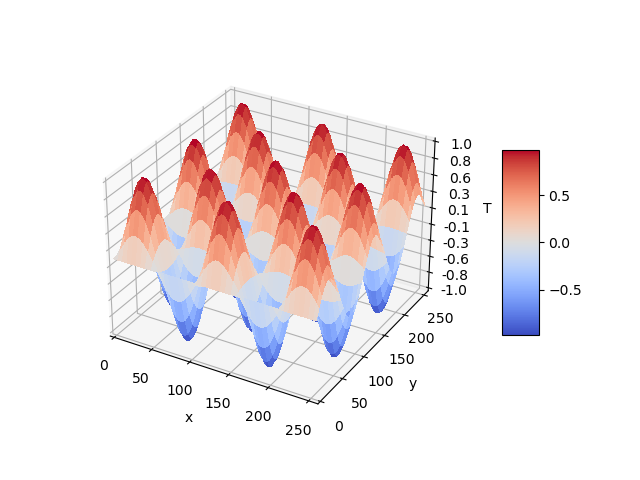
\includegraphics[scale=0.7]{global_0000.png}
    \caption{3D surface plot of temperature at iteration 0}
\end{figure}

\begin{figure}[h]
    \center
    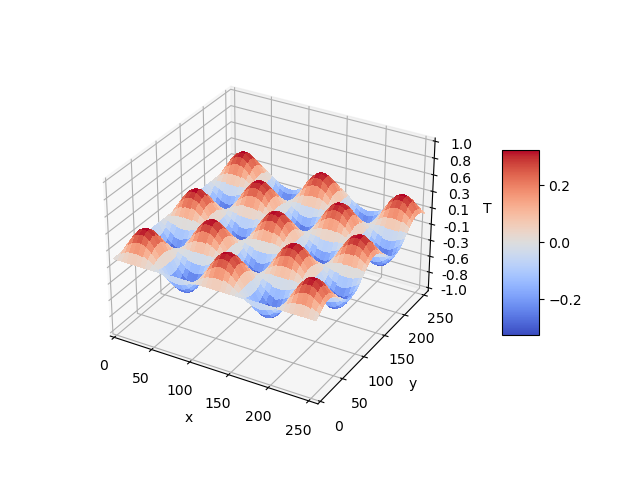
\includegraphics[scale=0.7]{global_1000.png}
    \caption{3D surface plot of temperature at iteration 1000}
\end{figure}

\begin{figure}[h]
    \center
    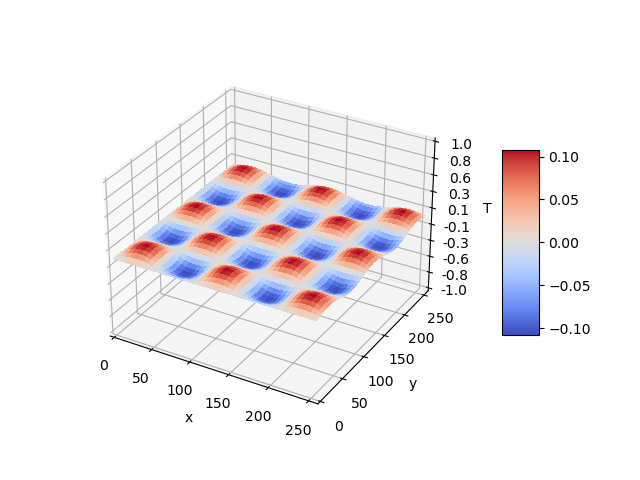
\includegraphics[scale=0.7]{global_2000.png}
    \caption{3D surface plot of temperature at iteration 2000}
\end{figure}

Performance in terms of both time (ms) and bandwidth (Gb/sec) are worse than
that observed for CPU computation. Console logs included below.


\paragraph{Problem 2: Implement global memory block kernel } Idea: re-write kernel to 
compute finite difference updates in blocks of size (blockDim.y * numYPerStep) 
* blockDim.x. It should still only use global memory.

In order to ensure each thread calculates at most numYPerStep updates, we add 
a for loop inside the kernel and carefully change thread block indexing for y 
dimension to be multiples of numYPerStep.

\begin{cpp}
/**
 * Kernel to propagate finite difference grid from the current
 * time point to the next.
 *
 * This kernel should be optimized to compute finite difference updates
 * in blocks of size (blockDim.y * numYPerStep) * blockDim.x. Each thread
 * should calculate at most numYPerStep updates. It should still only use
 * global memory.
 */
template<int order, int numYPerStep>
__global__
void gpuStencilBlock(float* next, const float* __restrict__ curr, int gx, int nx, int ny,
                    float xcfl, float ycfl) {
    
    
    int border = (int) (order / 2);
    int i = blockIdx.x * blockDim.x + threadIdx.x;
    int j = (blockIdx.y * blockDim.y + threadIdx.y)*numYPerStep;

    if (i < nx) {
	    int x = i + border;  // x coordinate of matrix
        int niter = min(numYPerStep, ny-j);  // number of updates thread computes
        for (int it = 0; it < niter; it++) {
            int y = j + it + border;
            int idx = gx * y + x;
            next[idx] = Stencil<order>(&curr[idx], gx, xcfl, ycfl);
        }
    }
}
\end{cpp}

Performance in terms of both time (ms) and bandwidth (Gb/sec) improved significantly
compared with \texttt{gpuStencilGlobal}. Console logs included below.


\paragraph{Problem 3: Plot bandwidth by grid size } Idea: want to understand how the 
different algorithms perform in terms of bandwidth as we increase the scale of the 
problem (grid size).

To do this, we fixed iterations to be 400 and used the following grid sizes: 
256 x 256; 512 x 512; 1024 x 1024; 2048 x 2048; 4096 x 4096.

\begin{figure}[h]
    \center
    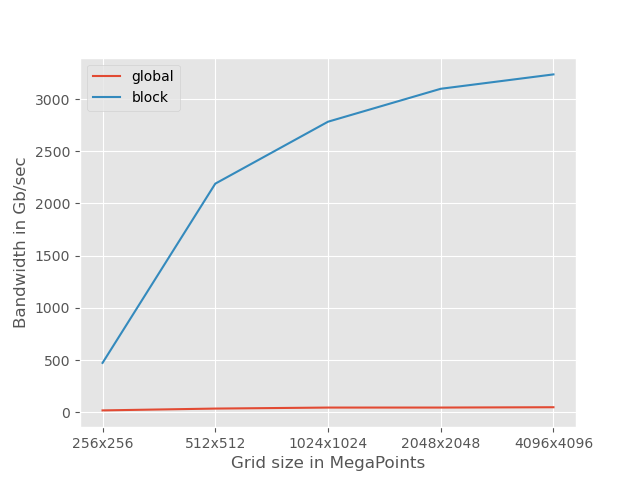
\includegraphics[scale=0.7]{bandwidth_by_alg_ord8.png}
    \caption{Plot of bandwidth vs grid size for different algorithms at order 8}
\end{figure}

...
...

\begin{figure}[h]
    \center
    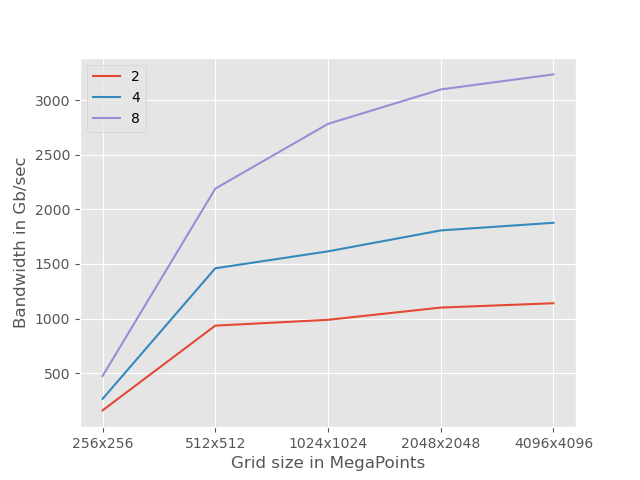
\includegraphics[scale=0.7]{bandwidth_by_order_block.png}
    \caption{Plot of bandwidth vs grid size for block algorithm at orders 2, 4 and 8}
\end{figure}

...
...


\paragraph{Problem 4: Explain performance results } For my implementation, the block
kernel for order 8 stencil achieved the best bandwidth (Gb/sec). 

Bandwidth is number of memory accesses divided by total execution time. In general, 
as you increase the number of warps requesting memory, you hide the latency of 
the memory pipe.

\begin{itemize}
    \item \textbf{Difference among kernels. } ...

    \item \textbf{Difference from varying order. } As you increase stencil order, 
    you increase the number of memory access requests for each warp to complete its 
    task. This hides latency and improves bandwidth.

    \item \textbf{Difference from varying problem size. } As you increase grid size, 
    you increase the number of warps requesting memory, which hides latency and 
    improves our bandwidth. This improvement will asymptotically approach the 
    compute bound of our hardware.

\end{itemize}


\paragraph{Problem 5: Implement shared memory block kernel } Idea: copy across current 
array values into shared memory to reduce access requests to global memory. We do this 
at the thread block level since we are guaranteed warps within a thread block share the 
same SM and therefore shared memory. Kernel logic included below.

Note, one challenge we need to work around is that each thread block needs to be able to 
access more values from the current array than it updates. This means our shared memory 
blocks are necessarily overlapping to ensure we update the whole array.

\begin{cpp}
/**
* Kernel to propagate finite difference grid from the current
* time point to the next.
*
* This kernel should be optimized to compute finite difference updates
* in blocks of size side * side using shared memory.
*/
template<int side, int order>
__global__
void gpuStencilShared(float* next, const float* __restrict__ curr, int gx, int gy,
                float xcfl, float ycfl) {
    
    // map thread to global position
    //int i = blockIdx.x * blockDim.x + threadIdx.x;
    //int j = blockIdx.y * blockDim.y + threadIdx.y;
    int border = (int) (order / 2);
    int sub_square_side = side - 2*border;
    int i = blockIdx.x*sub_square_side + threadIdx.x;
    int j = blockIdx.y*sub_square_side + threadIdx.y;

    // load mesh grid into shared memory
    __shared__ float shared[side][side];
    shared[threadIdx.x][threadIdx.y] = curr[gx * j + i];
    __syncthreads();

    // apply stencil inside domain
    if (i >= border && i < (gx-border)) {
        if (j >= border && j < (gy-border)) {
    
        if (threadIdx.x >= border && threadIdx.x < (side-border) &&
            threadIdx.y >= border && threadIdx.y < (side-border)) {
        
            next[gx * j + i] = Stencil<order>(
                &shared[threadIdx.x][threadIdx.y], 
                gx, 
                xcfl, 
                ycfl);
            }
        }
    }

}
   
\end{cpp}


Console logs from executing our kernels for grid size $1024x1024$
at order 8 for 400 iterations.

\begin{verbatim}
Output from main
----------------
Order: 2, 1024x1024, 400 iterations
                     time (ms)     GBytes/sec
            CPU        169.085         59.534
         Global        606.715        16.5915
          Block        10.1822        988.616
         Shared        1.20602        8346.76
There were 1048576 total locations where there was a difference between the cpu and gpu

                         L2Ref           LInf          L2Err
         Global         0.2477              0              0
          Block         0.2477              0              0
         Shared         0.2477       0.507062       0.253675
\end{verbatim}


Submission information logs.
\begin{verbatim}
jelc@cardinal2:~$ /afs/ir.stanford.edu/class/cme213/script/submit.py hw3 private/cme213-jelc53/hw3
Submission for assignment 'hw3' as user 'jelc'
Attempt 2/10
Time stamp: 2022-05-01 21:36
List of files being copied:
    private/cme213-jelc53/hw3/main_q1.cu	 [13253 bytes]
    private/cme213-jelc53/hw3/recurrence.cuh	 [1589 bytes]
    private/cme213-jelc53/hw3/pagerank.cuh	 [5894 bytes]
    private/cme213-jelc53/hw3/benchmark.cuh	 [795 bytes]

Your files were copied successfully.
Directory where files were copied: /afs/ir.stanford.edu/class/cme213/submissions/hw3/jelc/2
List of files in this directory:
    main_q1.cu	 [13253 bytes]
    recurrence.cuh	 [1589 bytes]
    pagerank.cuh	 [5894 bytes]
    benchmark.cuh	 [795 bytes]
    metadata	 [137 bytes]

This completes the submission process. Thank you!
    
jelc@cardinal2:~$ ls /afs/ir.stanford.edu/class/cme213/submissions/hw3/jelc/2
benchmark.cuh  main_q1.cu  metadata  pagerank.cuh  recurrence.cuh
\end{verbatim}

\end{document}
